Avoiding obstacles is one of the most important tasks in robotics. To sucessfully complete 
a given task, a robot must avoid obstacles, stationery and moving.

Especially in Dynamic Movement Primitives where there exists an online change in trajectories, it seems fitting
to have an obstacle avoidance approach that evolves in time with the movement primitives. 
There exists many approaches to obstacle avoidance in movement primitives, and the one that we have implemented uses
dynamic potential field as an attraction-repulsion system, to avoid obstacles.

\section{Potential Fields for Obstacle Avoidance}
\subsection{Static Potential Fields}
The concept of the potential field was first introduced by Khatib\cite{khatibArtificial}. Here each obstacle acts as a repulsive potential field 
defined by Eq (\ref{eq:khatibField}). Hence the obstacle "exerts" a force on the robot, given by the gradient of the potential field,
i.e. $\vect{\varphi(x)} = -\nabla U(x)$.

\begin{equation}
    \label{eq:khatibField}
    U_{static}(\vect{x}) = 
    \begin{dcases}
        \ddfrac{\eta}{2} \left( \ddfrac{1}{p(\vect{x})} - \ddfrac{1}{p_0}\right)^2 & p(\vect{x}) \leq p_0 \\
        0 & p(\vect{x}) > p_0
    \end{dcases}
\end{equation}
where, $p_0$ is the radius of influence of the obstacle, and $\eta$ a constant gain paramerter.

This field is called the static potential field because it is not influenced by the obstacles and the robots velocity.
This robot external force is then added to the trandoformation system of DMP which can be written as:
\begin{equation}
    \tau \dot{z} = \alpha_z (\beta_z \left( z - z_g \right) - \dot{z}) + f(x) + \vect{\varphi(x,v)}
\end{equation}

This method did not allow for smooth obstacle avoidance as shown in \cite{peterOG}, and proposed a new method
which we implemented in this work.
\subsection{Dynamic Potential Fields}
The dynamic potential field is a function of the robots (or its end effectors) position $\vect{x}$ 
and velocity $\vect{v}$, hence the term \textit{dynamic}.

The dynamic potential field is defined to achieve the following properties:
\begin{itemize}
    \item The magnitude of the potential decreases with the distance from $\vect{x}$ to the obstacle.
    \item The magnitude of the increases with the increase in the robots velocity.
    \item The magnitude of the potential should increase with the 
    angle between the robot's velocity vector and the obstacle, and be zero if the angle is more than $90^{\circ}$.
\end{itemize}

Thus the formation can be formulated as:
\begin{equation}
    U_{dynamic}(\vect{x,v}) = 
    \begin{dcases}
        \lambda (- \cos \theta )^{\beta} \ddfrac{||\vect{v}||}{p(\vect{x})}  & \frac{\pi}{2} < \theta \leq \pi \\
        0 & 0 \leq \theta < \frac{\pi}{2}
    \end{dcases}
\end{equation}
where $\lambda$ is a constant for the strength of the field, $\beta$ is a hyperparameter. The angle $\theta$ is the angle
\begin{equation}
    \cos \theta  = \ddfrac{\vect{v}^T \vect{x}}{||\vect{v}|| \vect{p(x)}}
\end{equation}
between the current velocity $\vect{v}$ and the robot's position $\vect{x}$ relative to the obstacle, and $p(x)$ denotes 
the distance between the $\vect{x}$ and the obstacle.
The obstacle force as stated before is derived from a negative gradient of the potential field as
\begin{align}
    \vect{\varphi(x,v)} &= -\nabla U_{dynamic}(\vect{x,v}) \\  
    &=\lambda (- \cos \theta)^{\beta -1} \ddfrac{||\vect{v}||}{p(\vect{x})} 
    \left( \beta \nabla_x \cos \theta - \ddfrac{\cos \theta}{p(\vect{x})} \nabla_x p(\vect{x}) \right)\label{eq:dynamicForceField}
\end{align}
where,
\begin{align}
    \nabla_x p(\vect{x}) &= \ddfrac{\vect{x - x_{obstacle}}}{p(\vect{x})} \\
    \nabla_x \cos \theta &= \ddfrac{ p(\vect{x}) \vect{v}^T - \vect{v}^Tx .\nabla_x p(\vect{x}) }{||\vect{v}|| p^2(\vect{x})}
\end{align}

\section{Multiple Obstacle Avoidance}
The formulation described above is for a single point like obstacle. One advantage of this approach is that it can be 
easily extended to avoid multiple obstacles, simply by adding the force field of each obstacle. 
Thus for N obstacles, we can write
\begin{equation}
    \varphi_{total} = \sum\limits_{i=1}^N \varphi_{i}(\vect{x})
\end{equation}
where $\varphi_{i}$ is the force field of the $i^{th}$ obstacle given by Eq. \ref{eq:dynamicForceField}.
An important point to note is that this method, \textit{does not} gurantee the convergence to goal pose,
due to the presence of local minima in the potential field.

\section{Implementation and Results}
The above formulation like the previous results is implemented in Python and simulated in Pybullet.

\subsection{2D Obstacle Avoidance}
A minimum acceleration trajectory between the initial and goal position of [-3,2] to [3,-2] with an initial velocity of [-1,0]. The obstacle
is placed at the origin. The desired trajectory passes close to the obstacle and the force field from the obstacle makes sure that
the robot avoids the obstacle.

\begin{figure}[h]
    \centering
    \begin{subfigure}{0.5\textwidth}
        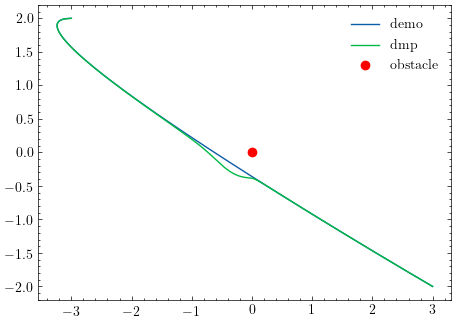
\includegraphics[width=1 \linewidth]{obsAvoid2D.png}
        \caption{2D Obstalce Avoidance}
        \label{fig:obsAvoid2D}
    \end{subfigure}%
    \begin{subfigure}{0.5\textwidth}
        \centering
        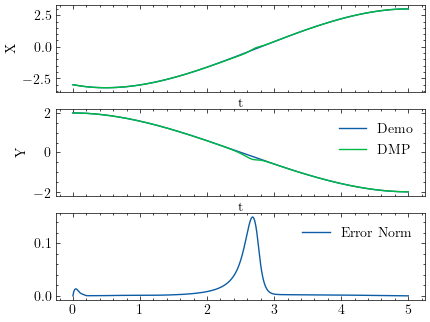
\includegraphics[width=1 \linewidth]{obsAvoid2D_error.png}
        \caption{Deviation from the desired trajectory}
        \label{fig:obsAvoid2D_error}
    \end{subfigure}
    \caption{Obstacle Avoidance in 2D and the deviation due to obstacle}
    \label{fig:obsAvoid2D_total}
\end{figure}

The graph in Figure \ref{fig:obsAvoid2D_error} shows the deviation from the demonstrated trajectory when the trajectory is close to the obstacle. 
\begin{figure}[!htp]
    \centering
    \begin{subfigure}{0.5\textwidth}
        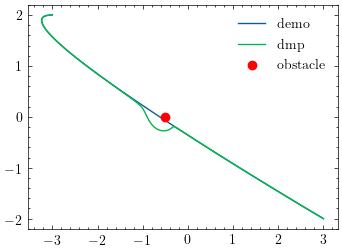
\includegraphics[width=1 \linewidth]{obsAvoid2D_error_1.png}
        \caption{2D Obstalce Avoidance}
        \label{fig:obsAvoid2D_1}
    \end{subfigure}%
    \begin{subfigure}{0.5\textwidth}
        \centering
        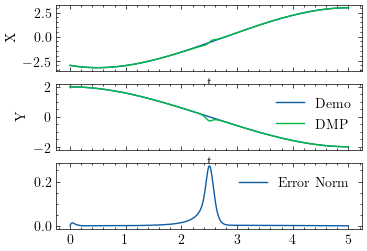
\includegraphics[width=1 \linewidth]{obsAvoid2D_1.png}
        \caption{Deviation from the desired trajectory}
        \label{fig:obsAvoid2D_error_1}
    \end{subfigure}
    \caption{Obstacle Avoidance in 2D and the deviation due to obstacle when the obstacle is very close to the demonstrateed trajcetory}
    \label{fig:obsAvoid2D_ontraj}
\end{figure}


This same effect is magnified when the obstacle is \textit{on} the demostrated trajectory, 
which is shown in Figure \ref{fig:obsAvoid2D_ontraj}, where
the obstacle was placed at [-0.5,0]. As mentioned in the formulation that we want the force field to decrese with the distance from the obstacle, which
is the case when the obstacle is placed at [2,1.5]. In this case their is litte to no deviation from the demostrated trajectory
as demonstrated in Figure \ref{fig:obsAvoid2Dfar}. The parameters for the dynamic potential field were $\lambda = 10 \text{ and } \beta = 2$
\begin{figure}[!htp]
    \centering
    \begin{subfigure}{0.5\textwidth}
        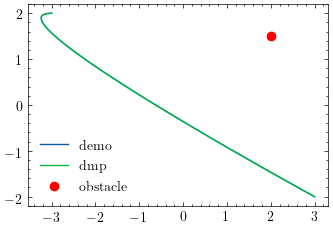
\includegraphics[width=1 \linewidth]{obsAvoidFar.png}
        \caption{2D Obstalce Avoidance when the obstacle is far away}
        \label{fig:obsAvoid2D_far}
    \end{subfigure}%
    \begin{subfigure}{0.5\textwidth}
        \centering
        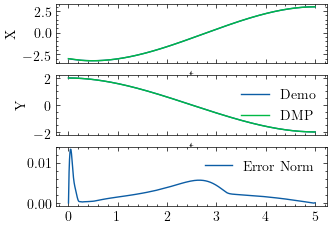
\includegraphics[width=1 \linewidth]{obsAvoidFar_error.png}
        \caption{Deviation from the desired trajectory}
        \label{fig:obsAvoid2D_error_far}
    \end{subfigure}
    \caption{Obstacle Avoidance in 2D and the deviation due to obstacle when the obstacle is far away from the demonstrateed trajcetory}
    \label{fig:obsAvoid2Dfar}
\end{figure}
\subsubsection{Moving Obstacle Avoidance} 
To demonstrate the ability to avoid moving obstacles, an obstacle is placed at origin and is moved with a constant velocity of [-0.1,-0.1],
with the parameter $\lambda = 10 \text{ and } \beta = 2$. The demonstrated trajectory is kept the same. The results of which can be seen below.

\begin{figure}[!htp]
    \centering
    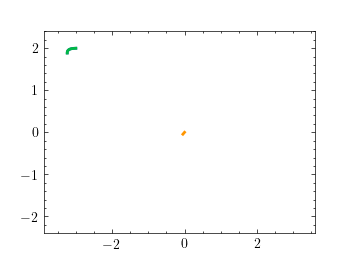
\includegraphics[width= 0.4 \textwidth]{animation_500.png}\quad
    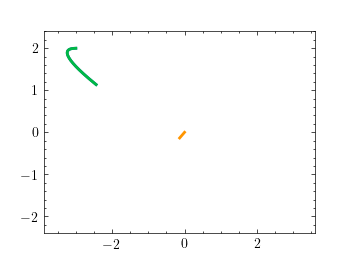
\includegraphics[width= 0.4 \textwidth]{animation_1500.png}\quad
    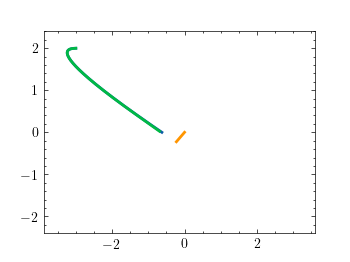
\includegraphics[width= 0.4 \textwidth]{animation_2500.png}

    \medskip

    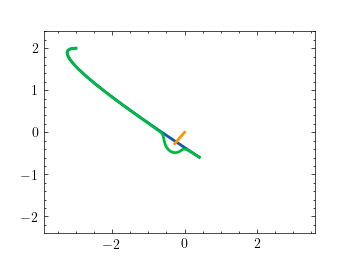
\includegraphics[width= 0.4 \textwidth]{animation_3000.png}\quad
    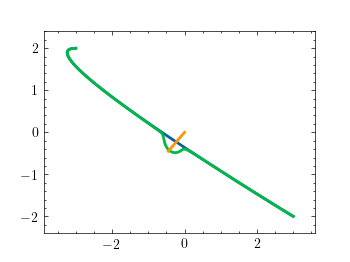
\includegraphics[width= 0.4 \textwidth]{animation_5000.png}

    \caption{2D obstacle avoidance of moving obstacles}
    \label{fig:2D_moveObs}
\end{figure}
The green path is the trajectory simulated by the DMP to follow the blue demonstrated trajectory, whereas the orange path is the path of the obstacle.




\subsection{Task Space Obstacle Avoidance}
The similar structure used in the planar case is used in the task space. A minimum acceleration trajectory is demonstrated 
between the points [3,2,3] to [-4,-5,-3] with an initial velocity of [-1,0,-1.3], where the obstacle is placed at the origin. The 
parameters for the potential field in this case are, $\lambda = 5 \text{ and } \beta = 2$.

\begin{figure}[!htp]
    \centering
    \begin{subfigure}{0.5\textwidth}
        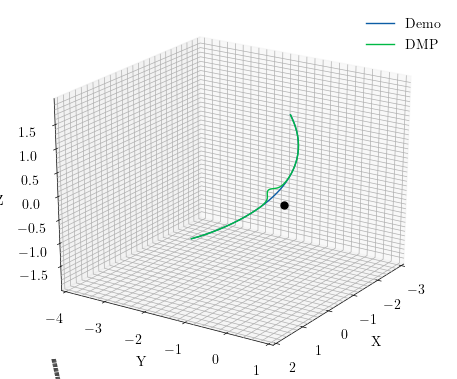
\includegraphics[width=1 \linewidth]{obsAvoid3D.png}
        \caption{3D Obstalce Avoidance}
        \label{fig:obsAvoid3D}
    \end{subfigure}%
    \begin{subfigure}{0.5\textwidth}
        \centering
        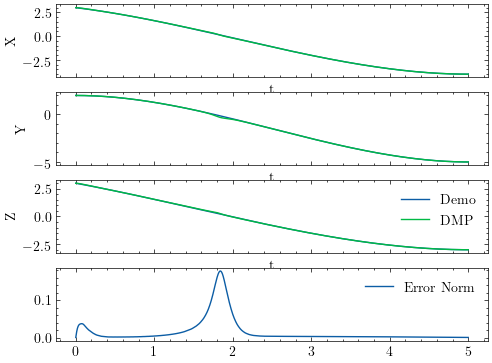
\includegraphics[width=1 \linewidth]{obsAvoid3D_error.png}
        \caption{Deviation from the desired trajectory}
        \label{fig:obsAvoid3D_error}
    \end{subfigure}
    \caption{Obstacle Avoidance in 3D and the deviation due to obstacle from the demonstrateed trajcetory}
    \label{fig:obsAvoid3Dfar}
\end{figure}

This implementation of 3D obstacle avoidance is also implemented on Pybullet, where we avoid a spherical obstacle
placed near the origin at [0,0.03,0.65] on a table, where we move the end-effector of the robot from [-0.3,0.2,0.71] to [0.3,-0.2,0.71].
The robot as mentioned before is controlled via velocity control. The results of the simulation can be seen below.
\begin{figure}[!htp]
    \centering
    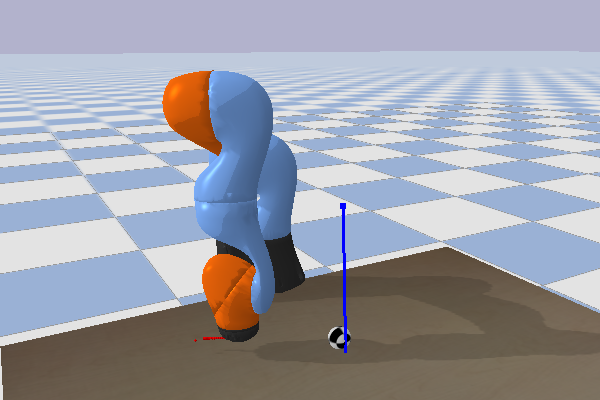
\includegraphics[width= 0.3 \textwidth]{singlePB1_cropped.png}\quad
    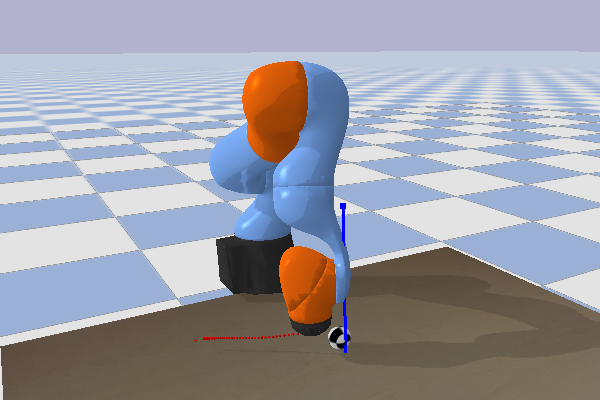
\includegraphics[width= 0.3 \textwidth]{singlePB2_cropped.png}\quad
    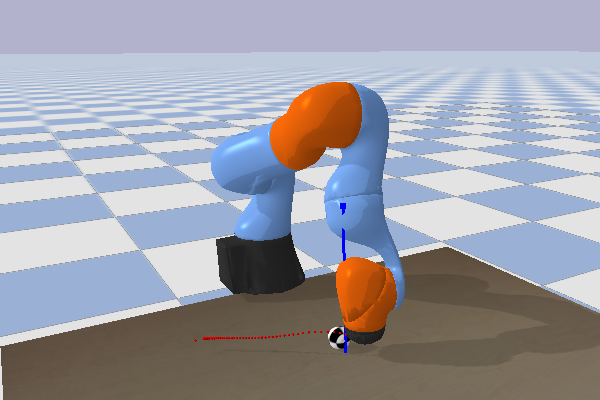
\includegraphics[width= 0.3 \textwidth]{singlePB3_cropped.png}

    \medskip

    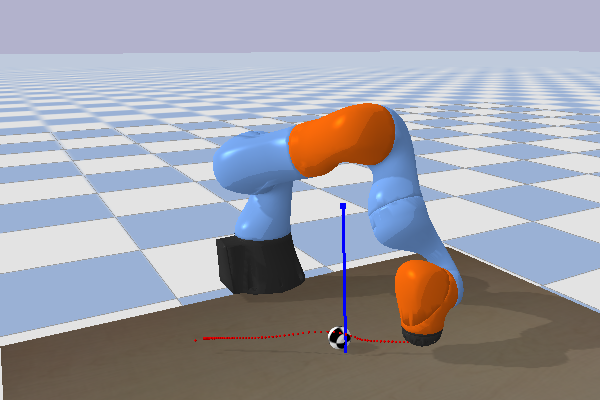
\includegraphics[width= 0.3 \textwidth]{singlePB4_cropped.png}\quad
    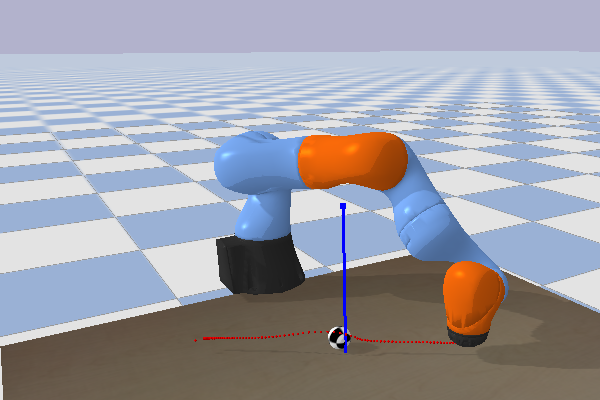
\includegraphics[width= 0.3 \textwidth]{singlePB5_cropped.png}

    \caption{3D obstacle avoidance of obstacles in Pybullet}
    \label{fig:pybulletsingleObs}
\end{figure}

\subsubsection{Multiple Obstacle Avoidance}
As described in the section, multiple point like obstacles can be avoided via the same formulation. The result 
of this extended formulation is shown below.

\begin{figure}[!htp]
    \centering
    \begin{subfigure}{0.5\textwidth}
        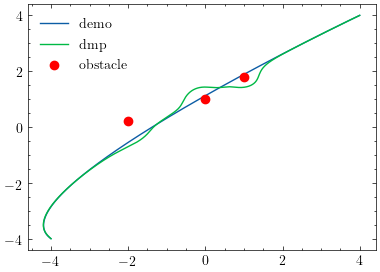
\includegraphics[width=1 \linewidth]{multiObs2D_traj.png}
        \caption{2D multiple obstacle avoidance}
    \end{subfigure}%
    \begin{subfigure}{0.5\textwidth}
        \centering
        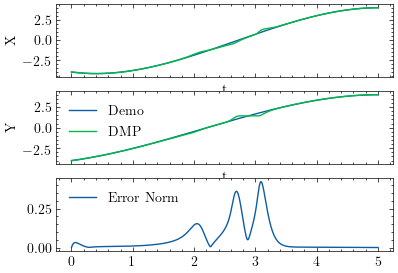
\includegraphics[width=1 \linewidth]{multiObs2D_error.png}
        \caption{Deviation from the desired trajectory}
    \end{subfigure}
    \caption{Obstacle Avoidance in 2D and the deviation due to multiple obstacles from the demonstrateed trajcetory}
\end{figure}

The same formulation is also implemented in PyBullet, the results of which is shown below.
\begin{figure}[!htp]
    \centering
    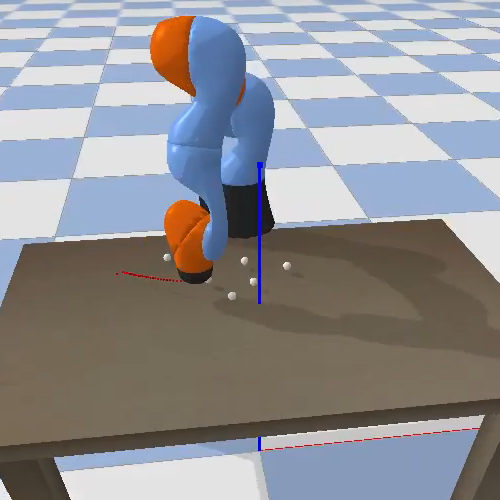
\includegraphics[width= 0.3 \textwidth]{multi_1_cropped.png}\quad
    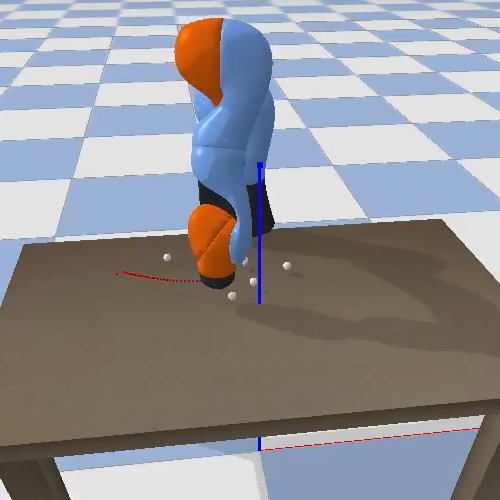
\includegraphics[width= 0.3 \textwidth]{multi_2_cropped.png}\quad
    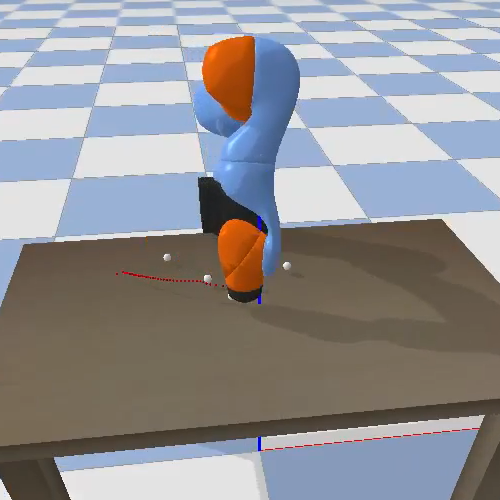
\includegraphics[width= 0.3 \textwidth]{multi_3_cropped.png}

    \medskip

    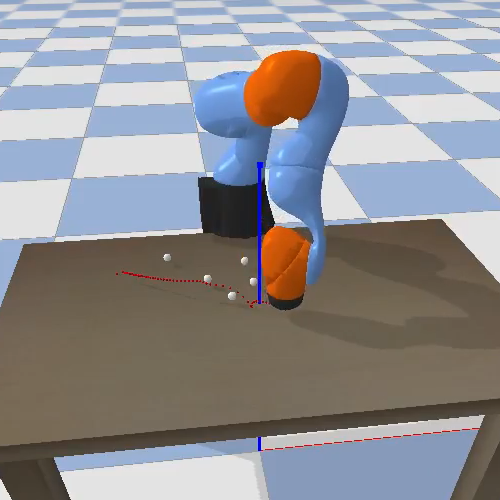
\includegraphics[width= 0.3 \textwidth]{multi_4_cropped.png}\quad
    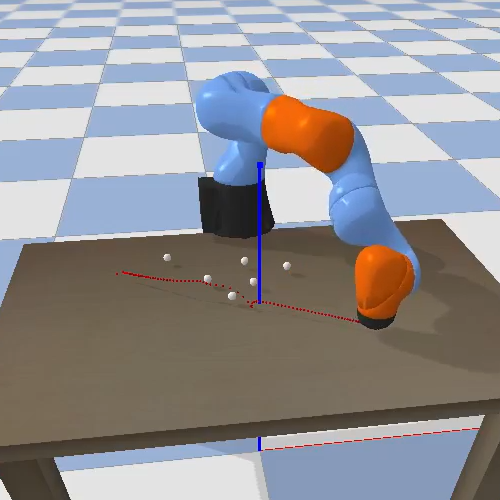
\includegraphics[width= 0.3 \textwidth]{multi_5_cropped.png}

    \caption{3D obstacle avoidance of obstacles in Pybullet}
    \label{fig:pybulletsingleObs}
\end{figure}

\subsection{Effect of the parameters: $\lambda$ and $\alpha_z$}
The parameters $\lambda$ and $\alpha_z$ dictate the way the robot will move in presence of the force field from obstacles.

The effect of $\alpha_z$ is similar to that of a spring, where the stiffness of the movement is directly proportional to $\alpha_z$.
But the effect of $\lambda$ is interesting. As the value of $\lambda$ increases, the strength of the force fields increases. But after a certain 
threshold value, the trajectory transversed by the robot will orbit around the obstacle. These effects of these parameters is
shown in the following figure Fig:\ref{fig:paramEffect}.

\begin{figure}[!htp]
    \centering
    \begin{subfigure}{0.5\textwidth}
        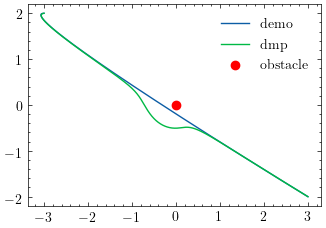
\includegraphics[width=1 \linewidth]{alpha_effect_20}
        \caption{DMP motion when $alpha_z = 20$}
        \label{fig:alpha_effect_20}
    \end{subfigure}%
    \begin{subfigure}{0.5\textwidth}
        \centering
        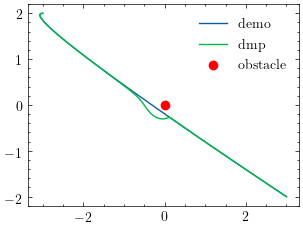
\includegraphics[width=1 \linewidth]{alpha_effect_50}
        \caption{DMP motion when $alpha_z = 50$}
        \label{fig:alpha_effect_50}
    \end{subfigure}
    \caption{Effect of $alpha_z$ on motion when avoiding obstacle}
    \label{fig:paramEffect}
\end{figure}

\begin{figure}[!htp]
    \centering
    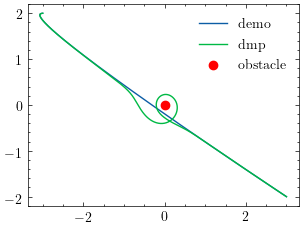
\includegraphics[width=0.6 \textwidth]{lambda_25.png}
    \caption{Effect of $\lambda$ on motion when avoiding obstacle, here $lambda = 25$. We can clearly see that the the motion is orbiting
    around the obstacle.}
\end{figure}




